\documentclass[12pt,a4paper,parskip]{scrartcl}
\usepackage[utf8]{inputenc}
\usepackage[T1]{fontenc}
\usepackage[ngerman]{babel}
\usepackage{lmodern}
\usepackage[babel,german=guillemets]{csquotes}
\usepackage[style=verbose-ibid,backend=bibtex8]{biblatex}
\bibliography{baclit280114}
\usepackage{amsmath}
\usepackage{amsfonts}
\usepackage{amssymb}
\usepackage{makeidx}
\usepackage{graphicx}
\usepackage{url}
\usepackage[locale=DE]{siunitx}%SI Einheiten etc.
\usepackage[german]{fancyref}%möglicherweise rausnehmen oder justieren
\usepackage{booktabs} %Tabellen Horizontale Linier dick darstellen
\usepackage{rotating}
\usepackage{lscape}
\usepackage{subfig}
\usepackage[left=3cm,right=3cm,top=2cm,bottom=2cm]{geometry}
\begin{document}
\subsection{Metallurgische Zusammenhänge}
In diesem Abschnitt wird erörtert was auf makroskopischer und mikroskopischer Ebene in metallischen Werkstoffen bei Formänderungsprozessen vor sich geht. Überdies soll ein Einblick gewonnen werden wie sich die verschiedenen Einflussgrößen während eines Umformvorgangs gegenseitig beeinflussen.
\subsubsection{Kristallaufbau}
In der Umformtechnik werden zum Großteil metallische Bauteile erzeugt. Eisen- wie Nichteisenmetalle bestehen aus metallisch gebundenen Atomen. Sie bekommen ihren Zusammenhalt aus einer sie gleichmäßig umgebenden frei beweglichen Elektronengaswolke, die aus abgegebenen Valenzelektronen besteht und so die positiven Metallionen  durch die sogenannte \emph{Metallbindung} bindet.\footcite[Vgl.][12]{wki} Ihr wichtigstes Merkmal ist der kristalline Aufbau. Darunter versteht man die feste, regelmäßige Struktur der Atome. In der Physik sowie in der Chemie existieren verschiedene Modelle über den Aufbau und das Aussehen solcher Kristallgebilde. In \fref{fig:makromikro}\footcite[Vgl.][4]{fu} wird eine Elementarzelle des $\alpha $-Eisen unter mikroskopischen (atomistischen) und makroskopischen Gesichtspunkten dargestellt. Oben rechts im Bild sind die drei Elementarzellen abgebildet aus denen Metalle zusammengesetzt sind. Es handelt sich um die  kubisch-raumzentrierte , kubisch-flächenzentrierte und hexagonale (das hdP steht für hexagonal dichteste Packung) Elementarzellen.\footcite[Vgl.][3-5]{fu}
\begin{figure}[hbtp]
\centering
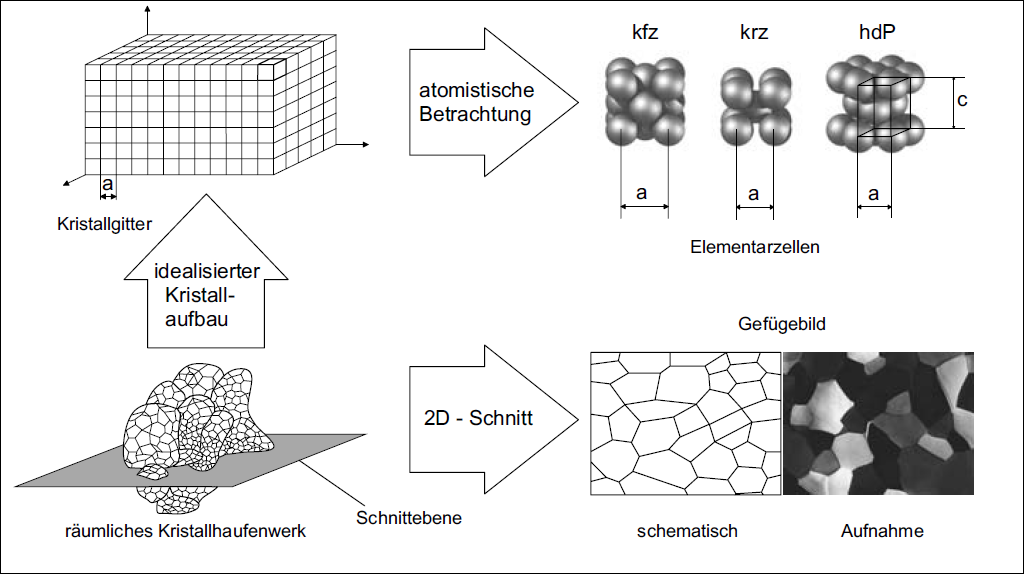
\includegraphics[scale=.54]{makromikro}
\caption{Aufbau eines Kristllgitter mikroskopisch (atomistisch) und makroskopisch.}
\label{fig:makromikro}
\end{figure}
Das kleinste Kristall im Metallgitterverband ist das sogenannte \emph{Einkristall} (siehe \fref{fig:elementarzellen})\footcite[Vgl.][37]{hu} es besitzt folgende Merkmale\begin{itemize}
\item allseitig freie Oberfläche
\item keine Korngrenzen
\item Fehlstellen wie z.B. Leerstellen, Versetzungen
\item anisotropisches Verhalten wegen bevorzugter Gleitrichtungen. Unter \emph{Anisotropie} wird das Auftreten von unterschiedlichen mechanischen und physikalischen Eigenschaften in die verschiedenen Raumrichtungen verstanden (z.B. Sperrholz). Im Gegensatz dazu weist \emph{isotropisches} Verhalten gleiche mechanische und physikalische Eigenschaften in die verschiedenen Raumrichtungen auf (z.B. Sonnenlicht)\footcite[vgl.][37]{hu}
\begin{figure}[hbtp]
\caption{Elementzarzellen (Einkristalle)}
\centering
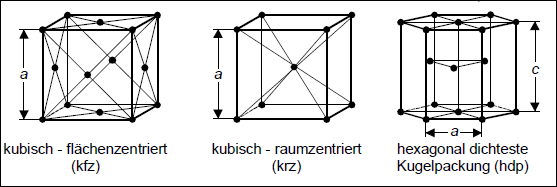
\includegraphics[scale=1]{elementarzellen}
\label{fig:elementarzellen}
\end{figure}

\end{itemize}
Die kleinste geometrisch zusammenhängende Einheit eines Kristallgitters ist die Elementarzelle. Knüpft man hypothetisch, in Richtung aller drei Koordinatenrichtungen, Elementarzellen aneinander entsteht ein Kristallgitter (siehe \fref{fig:makromikro} oben links). Das geometrische Aneinanderreihen von Elementarzellen erzeugt \emph{Idealkristalle} (fehlerfreie Kristalle) die so in der Realität nicht vorhanden sind. In der Realität sind in einem Raumgitter der Metalle zahlreiche Gitterfehler vorhanden. Hier wird unterschieden in folgende signifikante Gitterfehler:
\begin{enumerate}
\item  \emph{Nulldimensionale Gitterfehler} (punktförmig):\begin{itemize}
\item \emph{Zwischengitteratome} liegen vor wenn Atome auf Zwischengitterplätzen angeordnet sind. 
\item \emph{Austausch- oder Substitutionsatome}. Die Atomplätze werden von Fremdatomen beansprucht.
\item \emph{Einlagerungsatome} entstehen wenn die Zwischengitterplätze von Fremdatomen vereinnahmt werden.
\item \emph{Leerstellen} treten auf wenn wenn einzelne Gitterplätze nicht von Atomen besetzt werden. Sie sind bedeutend bei thermisch aktivierten Diffusionsvorgängen.
\end{itemize}
\item \emph{Eindimensionale Gitterfehler} sind linienförmige Strukturfehler (Versetzungen)(siehe \fref{fig:versetzung})\footcite[Vgl.][50]{wk}.

\begin{figure}[hbtp]
\centering
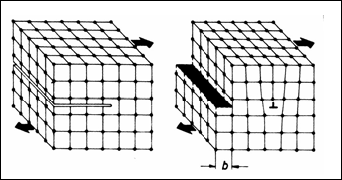
\includegraphics[scale=1.53]{versetzung}
\caption{Stufenversetzung}
\label{fig:versetzung}
\end{figure}
 Diese sind für Umformprozesse von übergeordnerter Bedeutung weil sie die plastische Formgebung besonders beeinflussen.
\item \emph{Zweidimensionale Gitterfehler} entstehen bei Oberflächendefekten. Die wichtigsten sind Korngrenzen und Phasengrenzflächen. Wenn ein Metall aus dem flüssigen Zustand kristallisiert wachsen die Keime zuerst an verschiedenen Stellen unabhängig voneinander. Im Laufe des Abkühlungsprozesses wachsen die Keim aufeinander zu und bilden Korngrenzen.
\end{enumerate}

Der Unterschied zwischen Real- und Idealkristallen ist in diesen Gitterfehlern begründet.Die Zugfestigkeit des Eisens liegt  z.B mehr als zwei Zehnerpotenzen unter der theoretisch Möglichen im Fall des Vorhandenseins eines Idealkristalls. Die Abstände der Atome sind in den Elementarzellen in verschiedene Richtungen unterschiedlich ausgeprägt. Das ist die Ursache für die Richtungsabhängigkeit bestimmter Eigenschaften der Metalle. Bestimmte Herstellungsverfahren (z.B. einige Walzverfahren, gerichtete Erstarrung) zielen darauf ab die Orientierung der Kristallite in eine bestimmte Richtung zu beeinflussen. Dieses Vorgehen bezeichnet man als Textur. Sie ermöglicht das die Werkstoffeigenschaften richtungsabhängig werden.  Die Richtungsabhängigkeit wird wie schon oben erwähnt mit dem Begriff der \emph{Anisotropie}. 
Während des Erstarrungsprozesses technischer Schmelzen werden Verunreinigungen überwiegend vor der Erstarrungsfront hergeschoben. Es bilden sich Ansammlungen von Verunreinigungen an den Korngrenzen. Ein reales Gefüge ist durch einen metallogfrafischen Schliff im Lichtmikroskop zu erkennen und mit einem schematischem Gefüge verglichen (siehe \fref{fig:makromikro}) . Es sind lediglich Größe, Anordnung und Form der Kristalle erkennbar zu machen. Die innere Struktur ist nicht sichtbar zu machen.\footcite[Vgl.][3-6]{fu}






\end{document}  